\documentclass[12pt, a4]{article}
\usepackage[english]{babel}
\usepackage[utf8x]{inputenc}
\usepackage{fullpage}
\usepackage{listings}
\usepackage{graphicx}
\usepackage{color}

%Syntax highlighting
\definecolor{blue-violet}{rgb}{0.54, 0.17, 0.89}
\definecolor{ao}{rgb}{0.0, 0.5, 0.0}
\definecolor{amaranth}{rgb}{0.9, 0.17, 0.31}
\definecolor{ballblue}{rgb}{0.13, 0.67, 0.8}
\definecolor{onyx}{rgb}{0.06, 0.06, 0.06}


\lstset{
  breaklines=true,                 % automatic line breaking only at whitespace
  captionpos=b,                    % sets the caption-position to bottom
  breakatwhitespace=false,
  keepspaces=true,
  numbers=left,
  numbersep=5pt,
  showspaces=false,
  showstringspaces=false,
  showtabs=false,
  tabsize=4,  
  backgroundcolor=\color{white},   % choose the background color
  commentstyle=\color{ao},    % comment style
  keywordstyle=\color{amaranth},    % keyword style
  stringstyle=\color{blue-violet},    % string literal style
  numberstyle=\tiny\color{ballblue},	   % number style
  basicstyle=\ttfamily\footnotesize\color{onyx} % size of fonts used for the code
}

%Document Header
\title{\textbf{Department of CSE\\SSN College of Engineering}}
\author{\textbf{Vishakan Subramanian - 18 5001 196 - Semester VII}}
\date{05 September 2021}

\begin{document}
\maketitle
\hrule
\section*{\center{UCS 1712 - Graphics And Multimedia Lab}}
\hrule
\bigskip

%Assignment Details
\subsection*{\center{\textbf{Exercise 6: 2D Composite Transformations and Windowing in C++ using OpenGL}}}
\subsection*{\flushleft{Aim:}}
\begin{flushleft}

\begin{itemize}
\item To compute the composite transformation matrix for any 2 transformations given as input by the user and applying it on the object. The transformation can be any combination of the following:

	\begin{itemize}
	\item Translation
	\item Rotation
	\item Scaling
	\item Reflection
	\item Shearing 
	\end{itemize} 

Display the original and the transformed object.
Calculate the final transformation matrix by multiplying the two individual transformation matrices and then apply it to the object.

\textbf{Note:} Use Homogeneous coordinate representations and matrix multiplication to perform transformations. Divide the output window into four quadrants. (Use LINES primitive to draw x
and y axis)

\item Create a window with any 2D object and a different sized viewport. Apply window to viewport transformation on the object. Display both window and viewport. 

\end{itemize}
 
\end{flushleft}

%Code
\newpage
\subsection*{\flushleft{Code: 2D Composite Transformations:}}
\begin{flushleft}
\lstinputlisting[language = C++]{CompositeTransforms.cpp}
\end{flushleft}


%Output
\newpage
\subsection*{\flushleft{Output: Plot With Translation and Rotation}}
\begin{figure}[h]
\centering
\caption{Plot With Translation and Rotation.}
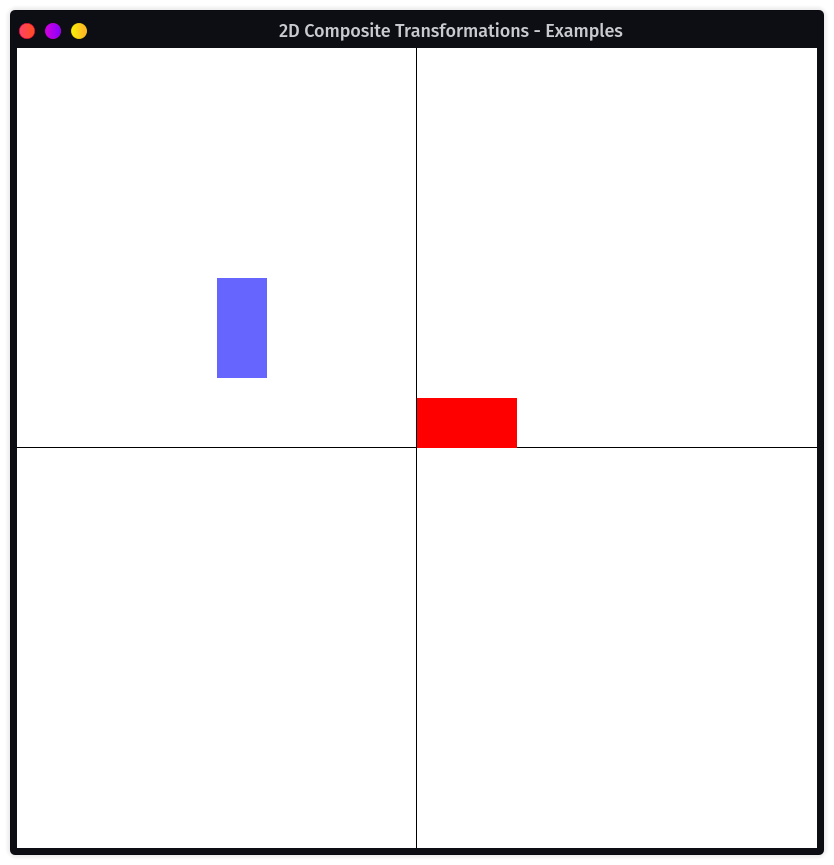
\includegraphics[height=15cm, width=15cm]{Outputs/Output-1.png}
\end{figure}

%Output
\newpage
\subsection*{\flushleft{Output: Console}}
\begin{figure}[h]
\centering
\caption{Output: Console.}
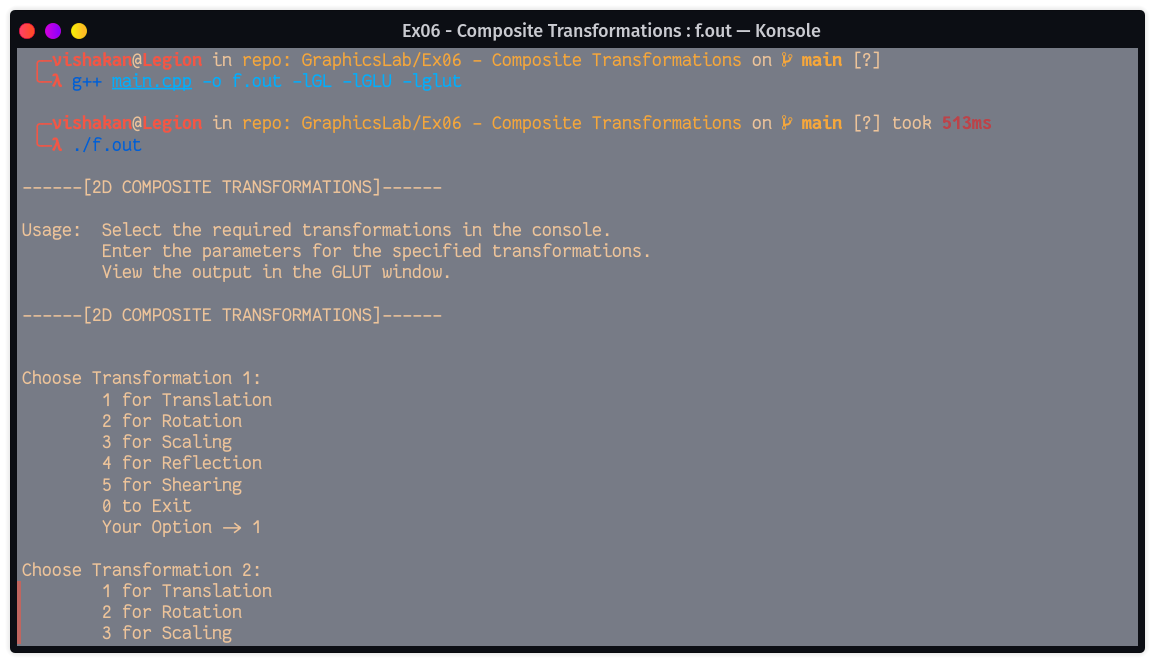
\includegraphics[height=12cm, width=17cm]{Outputs/Console-1.png}
\end{figure}

%Output
\newpage
\subsection*{\flushleft{Output: Console}}
\begin{figure}[h]
\centering
\caption{Output: Console.}
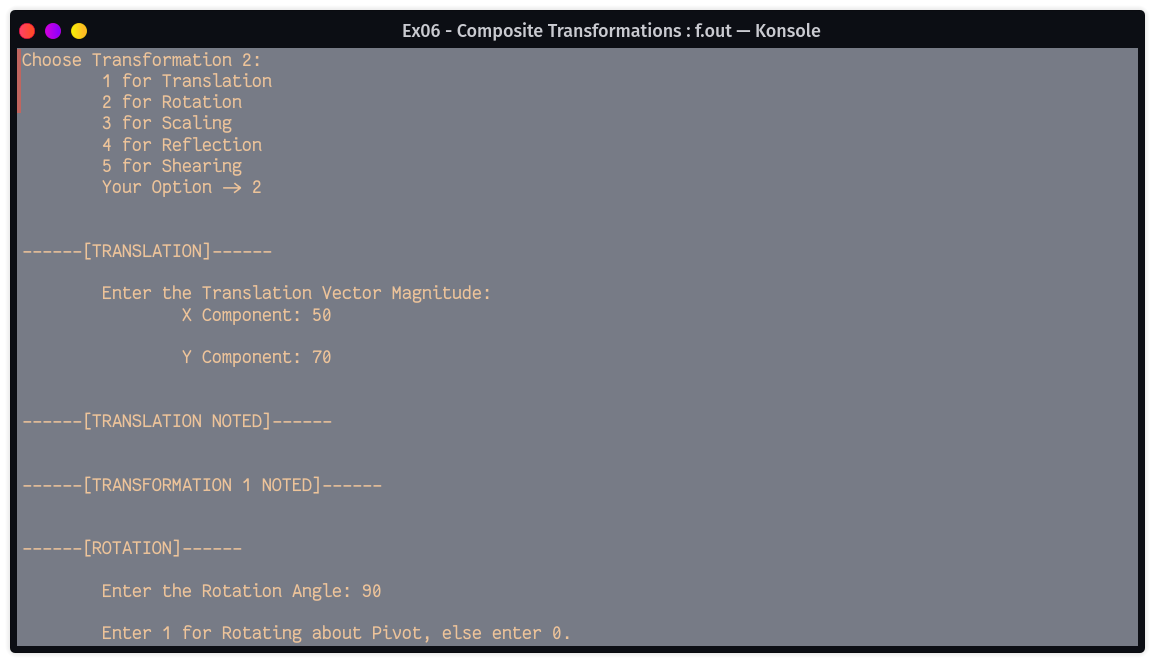
\includegraphics[height=12cm, width=17cm]{Outputs/Console-2.png}
\end{figure}

%Output
\newpage
\subsection*{\flushleft{Output: Console}}
\begin{figure}[h]
\centering
\caption{Output: Console.}
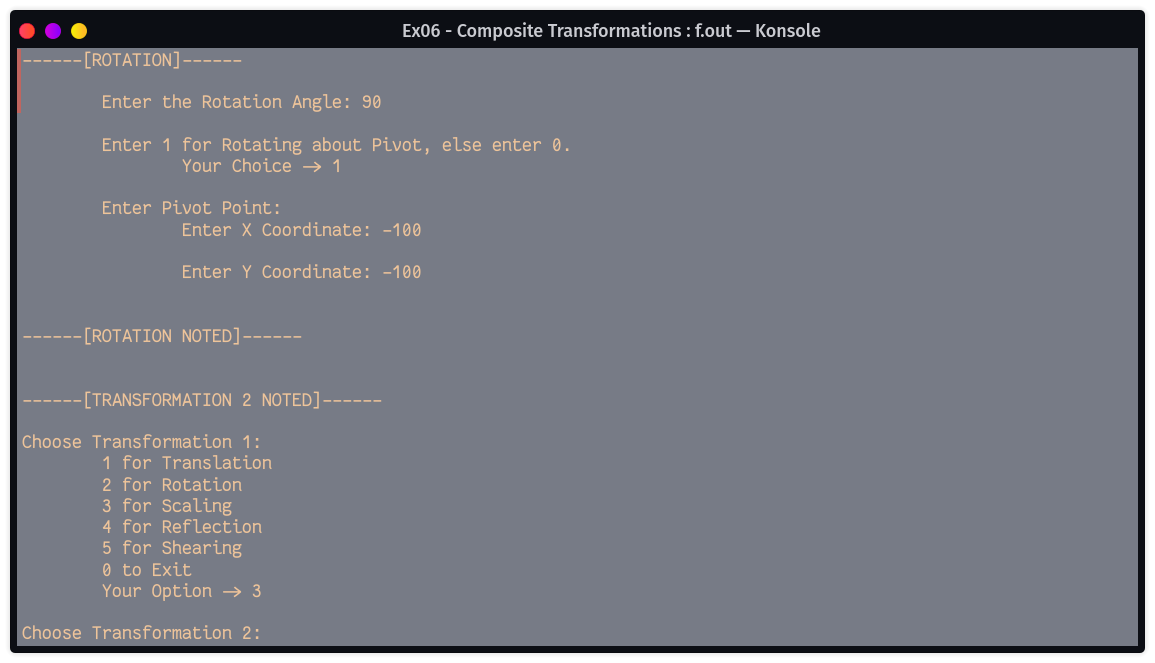
\includegraphics[height=12cm, width=17cm]{Outputs/Console-3.png}
\end{figure}

%Output
\newpage
\subsection*{\flushleft{Output: Plot With Scaling and Reflection}}
\begin{figure}[h]
\centering
\caption{Plot With Scaling and Reflection.}
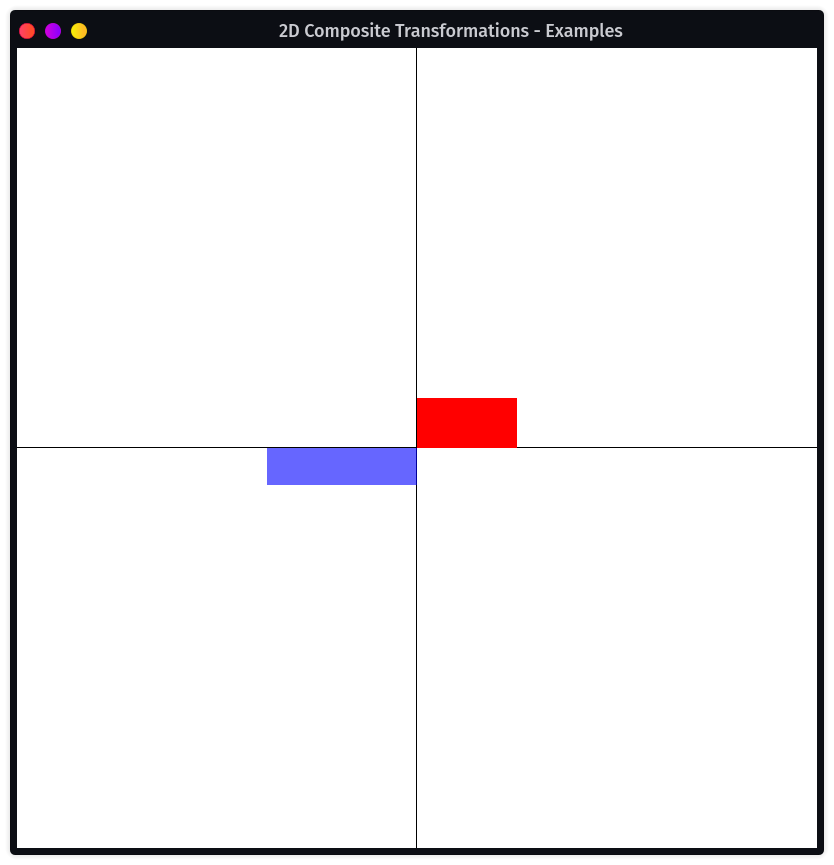
\includegraphics[height=15cm, width=15cm]{Outputs/Output-4.png}
\end{figure}

%Output
\newpage
\subsection*{\flushleft{Output: Console}}
\begin{figure}[h]
\centering
\caption{Console.}
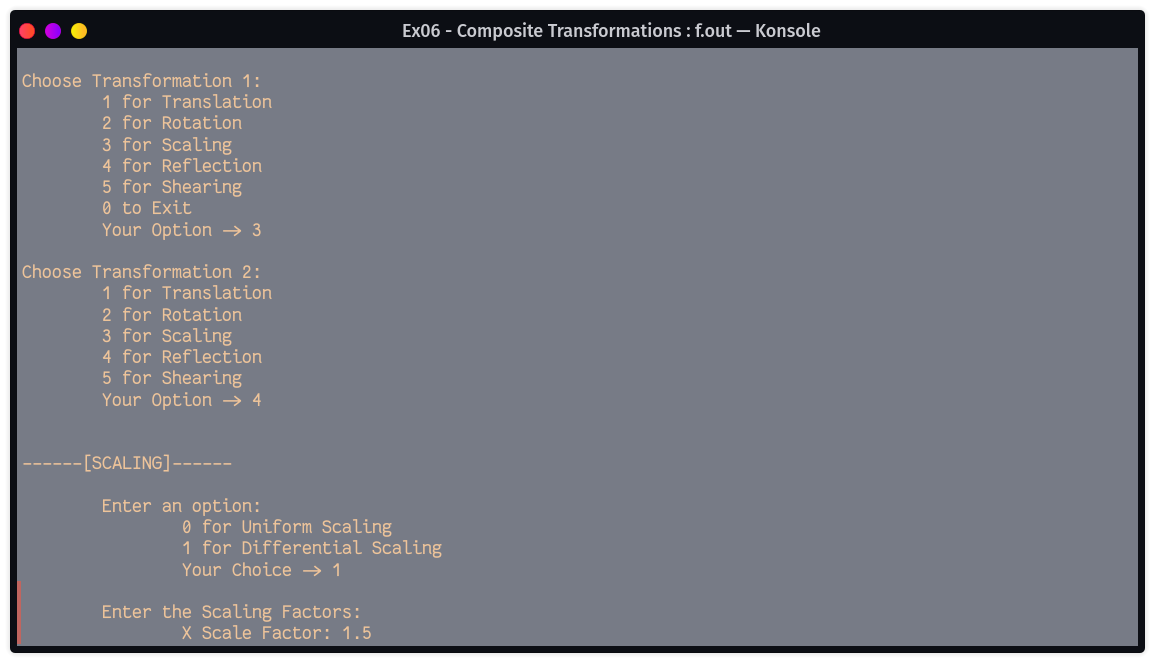
\includegraphics[height=12cm, width=17cm]{Outputs/Console-4.png}
\end{figure}

%Output
\newpage
\subsection*{\flushleft{Output: Console}}
\begin{figure}[h]
\centering
\caption{Console.}
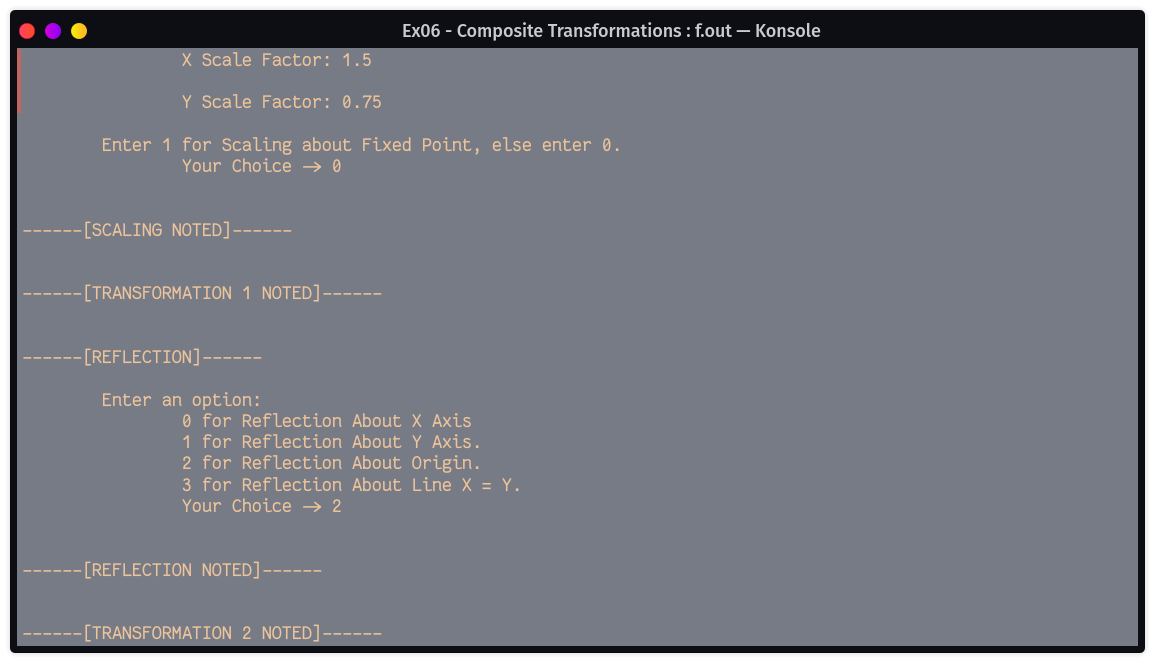
\includegraphics[height=12cm, width=17cm]{Outputs/Console-5.png}
\end{figure}

%Code
\newpage
\subsection*{\flushleft{Code: Window To Viewport Transformation:}}
\begin{flushleft}
\lstinputlisting[language = C++]{WindowToViewport.cpp}
\end{flushleft}


%Output
\newpage
\subsection*{\flushleft{Output: Window To Viewport Transformation}}
\begin{figure}[h]
\centering
\caption{Window To Viewport Transformation.}
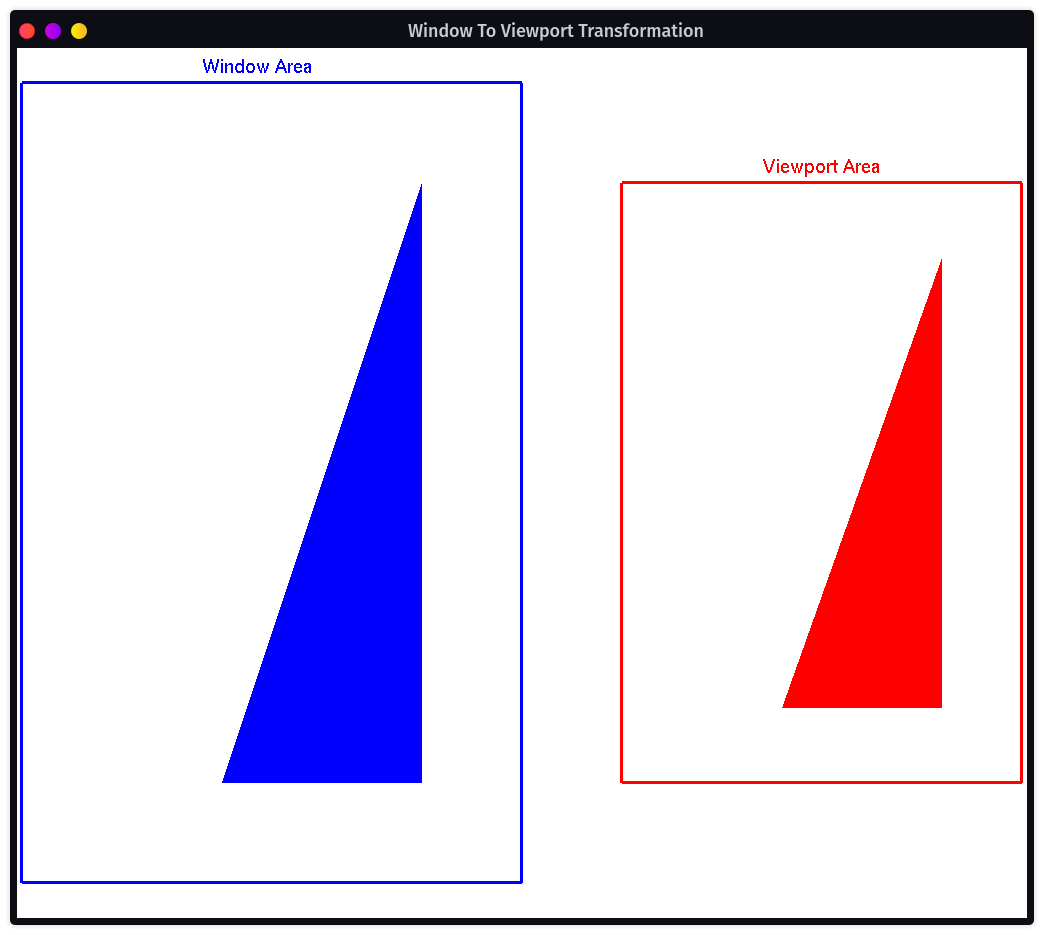
\includegraphics[height=15cm, width=15cm]{Outputs/Output-6.png}
\end{figure}



%Learning Outcome
\newpage
\subsection*{\flushleft{Learning Outcome:}}
\begin{itemize}
\item I understood how to perform \textbf{composite transformations} using OpenGL and C++ programming.
\item I learnt to perform proper matrix multiplication of the base transformation matrices to get the appropriate composite transformation matrix.
\item I applied the composite transformation on the base polygon and displayed the transformed polygon on the graph window. 
\item I learnt how to overcome the screen refreshing issue/asynchronous event handling while getting user I/O with the help of \textbf{glutTimerFunc()} and setting a \textbf{60 FPS} refresh rate.
\item I was able to perform composite transformations based on translation, rotation, scaling, reflection and shearing.
\item I learnt about \textbf{Window to Viewport Transformation}.
\item I learnt how to set up 2 windows, each to simulate a window and a viewport output window for the purpose of demonstrating the transformation.
\item I learnt to perform the transformation from window to viewport using \textbf{Translation \& Scaling} transformations.
\item I learnt the formula for performing the specific translation and scaling required for viewport transformation.
\item I understood how to display raster text using the \textbf{glutBitmapCharacter() and glRasterPos2d()} methods.
\item I refreshed my C/C++ concepts regarding \textbf{cin, cout and memcpy()} methods.
\item I learnt how to configure \textbf{OpenGL} in \textbf{Linux}.
\end{itemize}


\end{document}